\documentclass[
	12pt,
	a4paper,
	onepage,
	brazil
]{article}

\usepackage[brazil]{babel}
\usepackage[utf8]{inputenc}
\usepackage[T1]{fontenc}
\usepackage{lmodern}
\usepackage{hyperref}
\usepackage{amsmath}
\usepackage{amsthm}
\usepackage{amsfonts}
\usepackage{indentfirst}
\usepackage[most]{tcolorbox}
\usepackage{inconsolata}
\usepackage{caption}
\usepackage{floatrow}
\usepackage[lined,algonl,ruled]{algorithm2e}
\usepackage{float}
\usepackage{graphicx,url}
\usepackage{times,epsfig}
\usepackage[
	backend=bibtex8,
	style=numeric
]{biblatex}
\addbibresource{tp2.bib}
\usepackage{xcolor}
\hypersetup{
	colorlinks,
	linkcolor={red!50!black},
	urlcolor={red!80!black}
}



\usepackage{mathtools}
\DeclarePairedDelimiter\ceil{\lceil}{\rceil}

\sloppy

\author{Pedro Otávio Machado Ribeiro}
\title{Trabalho Prático 2\\Índice Invertido\\Algoritmos e Estruturas de Dados III - 2017/01}
\date{14/06/2017}

\begin{document}

	\maketitle
	
	\section{Introdução}
	
	Neste trabalho temos como contexto o rapaz Hetelberto Topperson que gosta muito de conversar no \textit{ZipZop}, porém ele possui uma memória seletiva e consegue lembrar do assunto que conversou com uma pessoa, mas não da pessoa. Hetelberto gostaria que o \textit{ZipZop} permitisse buscas que retornem o trecho de uma conversa com alguém dado um uma palavra qualquer. Dado isso, Hetelberto pediu ajuda para construir um índice invertido, já que sua amiga Inês implementara o buscador.
	
	O problema consiste em, dado $D$ arquivos de conversa de Hetelberto presentes num diretório $E$ e $M$ bytes de primária disponível, devemos escrever o índice invertido cada palavra de todos os arquivos em $M$ no arquivo \textit{index} dentro do diretório $S$. A solução do problema se resume a ordenar as palavras e obter os parâmetros que compões o índice invertido. Para resolver este problema, os seguintes são necessários:
	
	\subsection{Ordenação Interna}
	
	Dado que para realizar uma ordenação externa com um limite de memória primária dado, é necessário saber como ordenar valores armazenados na memória primária. Para isso, escolhi o \textit{Quicksort} para ordenar os dados. Para uma breve descrição sobre este método, veja \cite{quicksort-wiki}.
	
	\subsection{Índice Invertido}
	
	O índice invertido, conhecido também como índice remissivo, é conhecido popularmente como uma lista no final de livros, artigos, etc, de palavras seguidas de números referentes às páginas em que estas podem ser encontradas. No caso deste trabalho, o índice invertido será uma \textit{4-upla} representada por $I=\,<\,w,\,d,\,f,\,p\,>$, onde $w$ é a chave, no caso uma palavra, $d$ o número do arquivo em que ela se encontra, $f$ sua frequência no arquivo $d$ e $p$ sua posição em \textit{bytes} em relação ao início de $d$.
	
	\section{Metodologia}
	
	Para solucionar o problema foi necessário utilizar um método de ordenação externa. No caso de minha solução, escolhi o \textit{Mergesort} externo. Seja $D$ a quantidade de conversas, $M$ o tamanho da memória primária em \textit{bytes}, $E$ o diretório de conversas, $S$ o diretório onde o índice invertido deve ser armazenado, $T_I = 28$ o tamanho em \textit{bytes} da estrutura que armazena o índice ínvertido sem a frequência. Para solucionar o problema, os seguintes passos foram tomados:
	
	\begin{enumerate}
		\item Para cada arquivo de conversa, leia-se $C=M/T_I$ palavras até chegar ao final do arquivo, ordena-se todas as $C$ entradas em memória interna utilizando o \textit{Quicksort}, e finalmente escreve o resultado em um arquivo(página) temporário.
		\begin{enumerate}
			\item Toda vez que uma palavra é lida, sua posição em \textit{bytes} a partir do início é obtida e armazenada na estrutura de índice invertido, juntamente com o número do arquivo em que ela se encontra, que de antemão já sabemos qual é.
		\end{enumerate}
		\item Agora, para cada novo arquivo temporário já ordenado, realizo o \textit{merge} 2 a 2, até que ao final sobre apenas um arquivo, o qual possui todos índices invertidos, ainda sem a frequência, ordenados.
		\item Finalmente, no arquivo ordenado com todos índices invertidos parciais, duas passadas são feitas para obter a frequência de cada palavra em seu respectivo arquivo de conversa. Este procedimento é feito de forma que toda vez que uma uma chave diferente é encontrada, outro ponteiro do arquivo parte da primeira ocorrência da chave e vai andando até chegar a última, escrevendo cada uma no arquivo \textit{index} no diretório $S$ com sua respectiva frequência.
	\end{enumerate}
	
	\section{Complexidade}
	
	\subsection{Temporal}
	
	Seja $C=M/T_I$ a quantidade de palavras definida na seção anterior. As $C$ palavras são ordenadas utilizando o algoritmo \textit{Quicksort} que, no caso médio, possui complexidade $O(C\log C)$. Como nenhum outro processo, ignorando a leitura em arquivos, possui complexidade maior que isso, então a complexidade temporal será
	
	\begin{equation}
	O(C\log C)
	\end{equation}
	
	\subsection{Passadas}
	
	Temos $M$ como tamanho da memória principal. Podemos imaginar os arquivos de conversa como apenas um grande arquivo. Seja $T_a$ o tamanho do grande arquivo. Seja $N = T_a/M$ o número de páginas(subdivisões) de tamanho $M$ do grande arquivo. Como criamos um novo arquivo ordenado a partir de dois ordenados, o número de passadas diminui pela metade a cada iteração. Para cada \textit{merge} de arquivos realizado, lemos e escrevemos. Sabemos também que o merge das página é realizado em $O(N)$. Dessa forma, o número de passadas $P$ sobre o arquivo será: 
	\begin{equation}
	P=2N*(\ceil{\log_2 N} + 1)
	\end{equation}
	
	Assintóticamente, a complexidade será dada por:
	
	\begin{equation}
	O(N\log N)
	\end{equation}

	\subsection{Espacial}
	
	Como neste trabalho temos limite de memória interno dado por $M$, a complexidade espacial do programa será limitada superiormente por $M$, ou seja, a complexidade seria $O(M)$. Entretando, ao desenvolver o algoritmo, temos que utilizar as funções de manipulação de arquivo da linguagem \textit{C}, e estas utilizam a memória primária de forma que não temos controle.
	
	\section{Experimentos}
	
	Os testes foram realizados em meu computador pessoal, um notebook que não é mais um notebook, com as seguintes configurações:
	
	\begin{itemize}
		\item Sistema Operacional: Arch Linux
		\item Processador: Intel(R) Core(TM) i5-2430M CPU @ 4 $\times \ $2.40GHz
		\item Memória RAM: 6GB
	\end{itemize}
	
	Cada teste foi realizado 30 vezes e os valores apresentados é referente a média destes.
	
	Os casos de testes utilizados foram gerados utilizando um gerador de frases aleatórias \cite{lipsum} juntamente com uma ferramenta de textos \cite{texttool} que remove letras maiúsculas e pontuações.
	
	Optei por gerar 10 conversas aleatórias, cada uma com aproximadamente 88 \textit{bytes} de conteúdo, totalizando 888 \textit{bytes} de conversas. Para cada caso de teste, utilizei sempre as mesmas 10 conversas, variando apenas o tamanho da memória primária disponível, começando de 320 \textit{bytes} e dobrando até chegar em 163840 \textit{bytes}. Abaixo segue o gráfico do tempo em função do tamanho da memória primária:
	
	\begin{figure}[H]
		\centering
		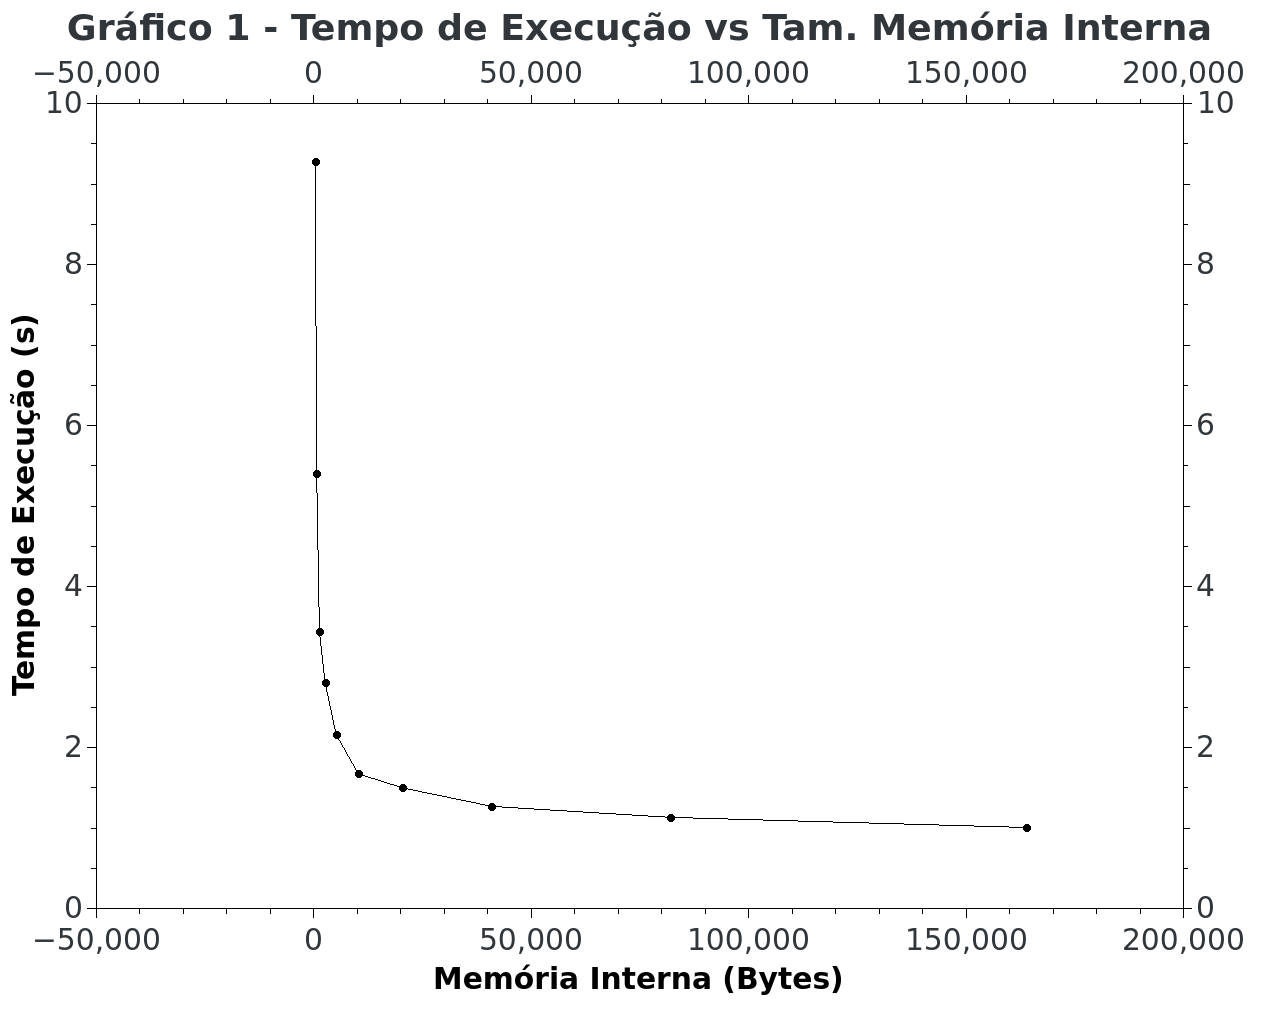
\includegraphics[scale=2.5]{Graph1.png}
		\caption{Tempo de Execução em função do tamanho da Memória Primária}
	\end{figure}
	
	\section{Análise de Resultado}
	
	Note que a cada vez que a memória primária disponível é dobrada, o tempo cai aproximadamente pela metade, pois o número de páginas(arquivos) criadas diminui pela metade, corroborando assim com a complexidade do problema. É possível perceber que em alguns intervalos não ocorre a diminuição do tempo pela metade. Isso ocorre possivelmente devido ao tempo de uso de meu notebook(6 anos), além de que outros programas também poderiam estar utilizando o disco ao mesmo tempo.
	
	\section{Conclusão}
	
	O objetivo do trabalho foi alcançado. O programa retorna para Hetelberto Topperson o índice ínvertido de todas conversas em conjunto devidamente ordenado.
	
	O problema de ordenação externo é um dos problemas clássicos da computação, e é amplamente utilizando em aplicações de \textit{database}, como a máquina de busca do \textit{Google} ou de qualquer outro buscador.
	
	No \textit{Mergesort} externo que implementei, utilizo apenas dois \textit{buffers} para fazer o \textit{merge} das páginas. Uma melhora que poderia ser feita neste programa é utilizar mais de dois \textit{buffers}, diminuindo mais ainda o tempo de execução do programa.
	
	\nocite{*}
	
	\printbibliography[title=Referências]

\end{document}